%! Author = giaco
%! Date = 16/05/2024

\section{Experiments \& Results}
\label{sec:experiments}
Regarding the experiments, we mainly used the Stable Baselines suite \cite{stable-baselines} and Gymnasium \cite{towers_gymnasium_2023} for our tests.
We decided to restrict our tests to only four environments, namely \textit{Pong, Breakout, Asteroids, and Ms. Pacman,} this was to avoid adding complexity and growing the time for experiments. We believe that this choice of games provides a fair compromise between simple games like Pong and much more complex games with lots of moving objects like Asteroids.
Furthermore, the choice of games was dictated by the availability of the RAM annotations provided in \cite{anand2019unsupervised}.
For each environment, we selected the \textit{NoFrameskip-v4} version of the game.

Our purpose was to change the representation learning part of PPO considering different skills to use and different ways of concatenating them, leaving the policy learning part as it is.

So, first of all, we needed a dataset on which to train the skills. For each environment, we then collected a dataset consisting of INSERIRE episodes using an agent playing randomly and preprocessing the game frames in the same way the agent would see them, thus in grayscale and of size 84x84 pixels.

Then, we defined a set of basic skills that are informative enough, so we chose the skills of Video Object Segmentation, Object Keypoints, and State Representation.
We implemented the three models as specified in their respective papers and used this newly created dataset to train the networks.
We then froze the weights of these skills and used them when training the agent.

A first round of experiments was conducted with the methods and parameters shown in Tab \ref{tab:firstround}.
Here we test all the concatenation methods shown in Sec. \ref{sec:extractors}, in this way we start to see which extractor works well for which game.
\begin{table}[htbp]
    \begin{center}
        \begin{tabular}{ll}
            \multicolumn{1}{l}{EXTRACTORS}  &\multicolumn{1}{l}{\bf PARAMETERS}
            \\ \hline \\
            Linear Concatenation              &  / \\
            Fixed Linear Concatenation        & 256, 512, 1024 \\
            CNN Concatenation                 & 1, 2, 3 \\
            Combine                           & / \\
            Reservoir Concatenation           & 512, 1024, 2048 \\
            Dot Product Attention             & 256, 512, 1024 \\
            Weights Sharing Attention         & 256, 512, 1024 \\

        \end{tabular}
    \end{center}
    \caption{This table shows the different configurations used for the extractors. For Fixed Linear Concatenation, Dot Product Attention, and Weights Sharing Attention the values indicate the fixed dimensions of skill embeddings and context. For Reservoir Concatenation, the values indicate the size of the reservoir. For CNN Concatenation the values indicate the number of convolutional layers.}
    \label{tab:firstround}
\end{table}

In the subsequent phase, the research progressed with a refined focus. We considered only the \textbf{three most effective} extractors identified from the initial experiments, and, if an extractor is already in the top 3, we consider the one immediately following with the best reward.
This strategic approach allowed for a deeper exploration of the performance nuances among the top contenders.
We provide a summary of the best extractors we chose for each game in Tab. \ref{tab:top3}.
As can be seen from the table at this stage, the best 3 agents for Breakout are missing because the agents failed to be competitive with a PPO agent and require a more in-depth study which will be done later.
For the execution of these experiments, a seed was set for reproducibility. We used the Atari Wrapper for each environment to preprocess the observations as standard procedure. Agents are trained for \textit{10.000.000} steps using the parameters provided by Stable Baselines in rl-zoo Github repository for Atari games considering PPO \cite{rl-zoo3}.
For each \textit{40,000} steps agents were evaluated for 100 episodes.

\begin{table}[htbp]
    \begin{center}
        \begin{tabular}{ll}
            \multicolumn{1}{l}{\bf GAME}  &\multicolumn{1}{l}{\bf EXTRACTORS}
            \\ \hline \\
            Pong       & Weights Sharing (1024), Reservoir (1024), CNN Concat. (2) \\
            Ms. Pacman & Weights Sharing (256), Reservoir (1024), CNN Concat. (2) \\
            Asteroids         & Reservoir (512), Reservoir (1024) \\
            Breakout          & Weights Sharing (256), Fixed Lin. Concat. (512), CNN Concat (3) \\
        \end{tabular}
    \end{center}
    \caption{In the table we see the extractors chosen for each game. The number in parentheses indicates the fixed embedding size for skills or context for the weights sharing extractor, the size of the reservoir for the reservoir extractor, and the number of convolutional layers for the CNN extractor.}
    \label{tab:top3}
\end{table}

Fig. \ref{fig:trainresults}, instead shows the learning curves of agents during training, the curves are smoothed using a running average.

\begin{figure}[htbp]
    \centering
    \begin{subfigure}[b]{0.32\textwidth}
        \centering
        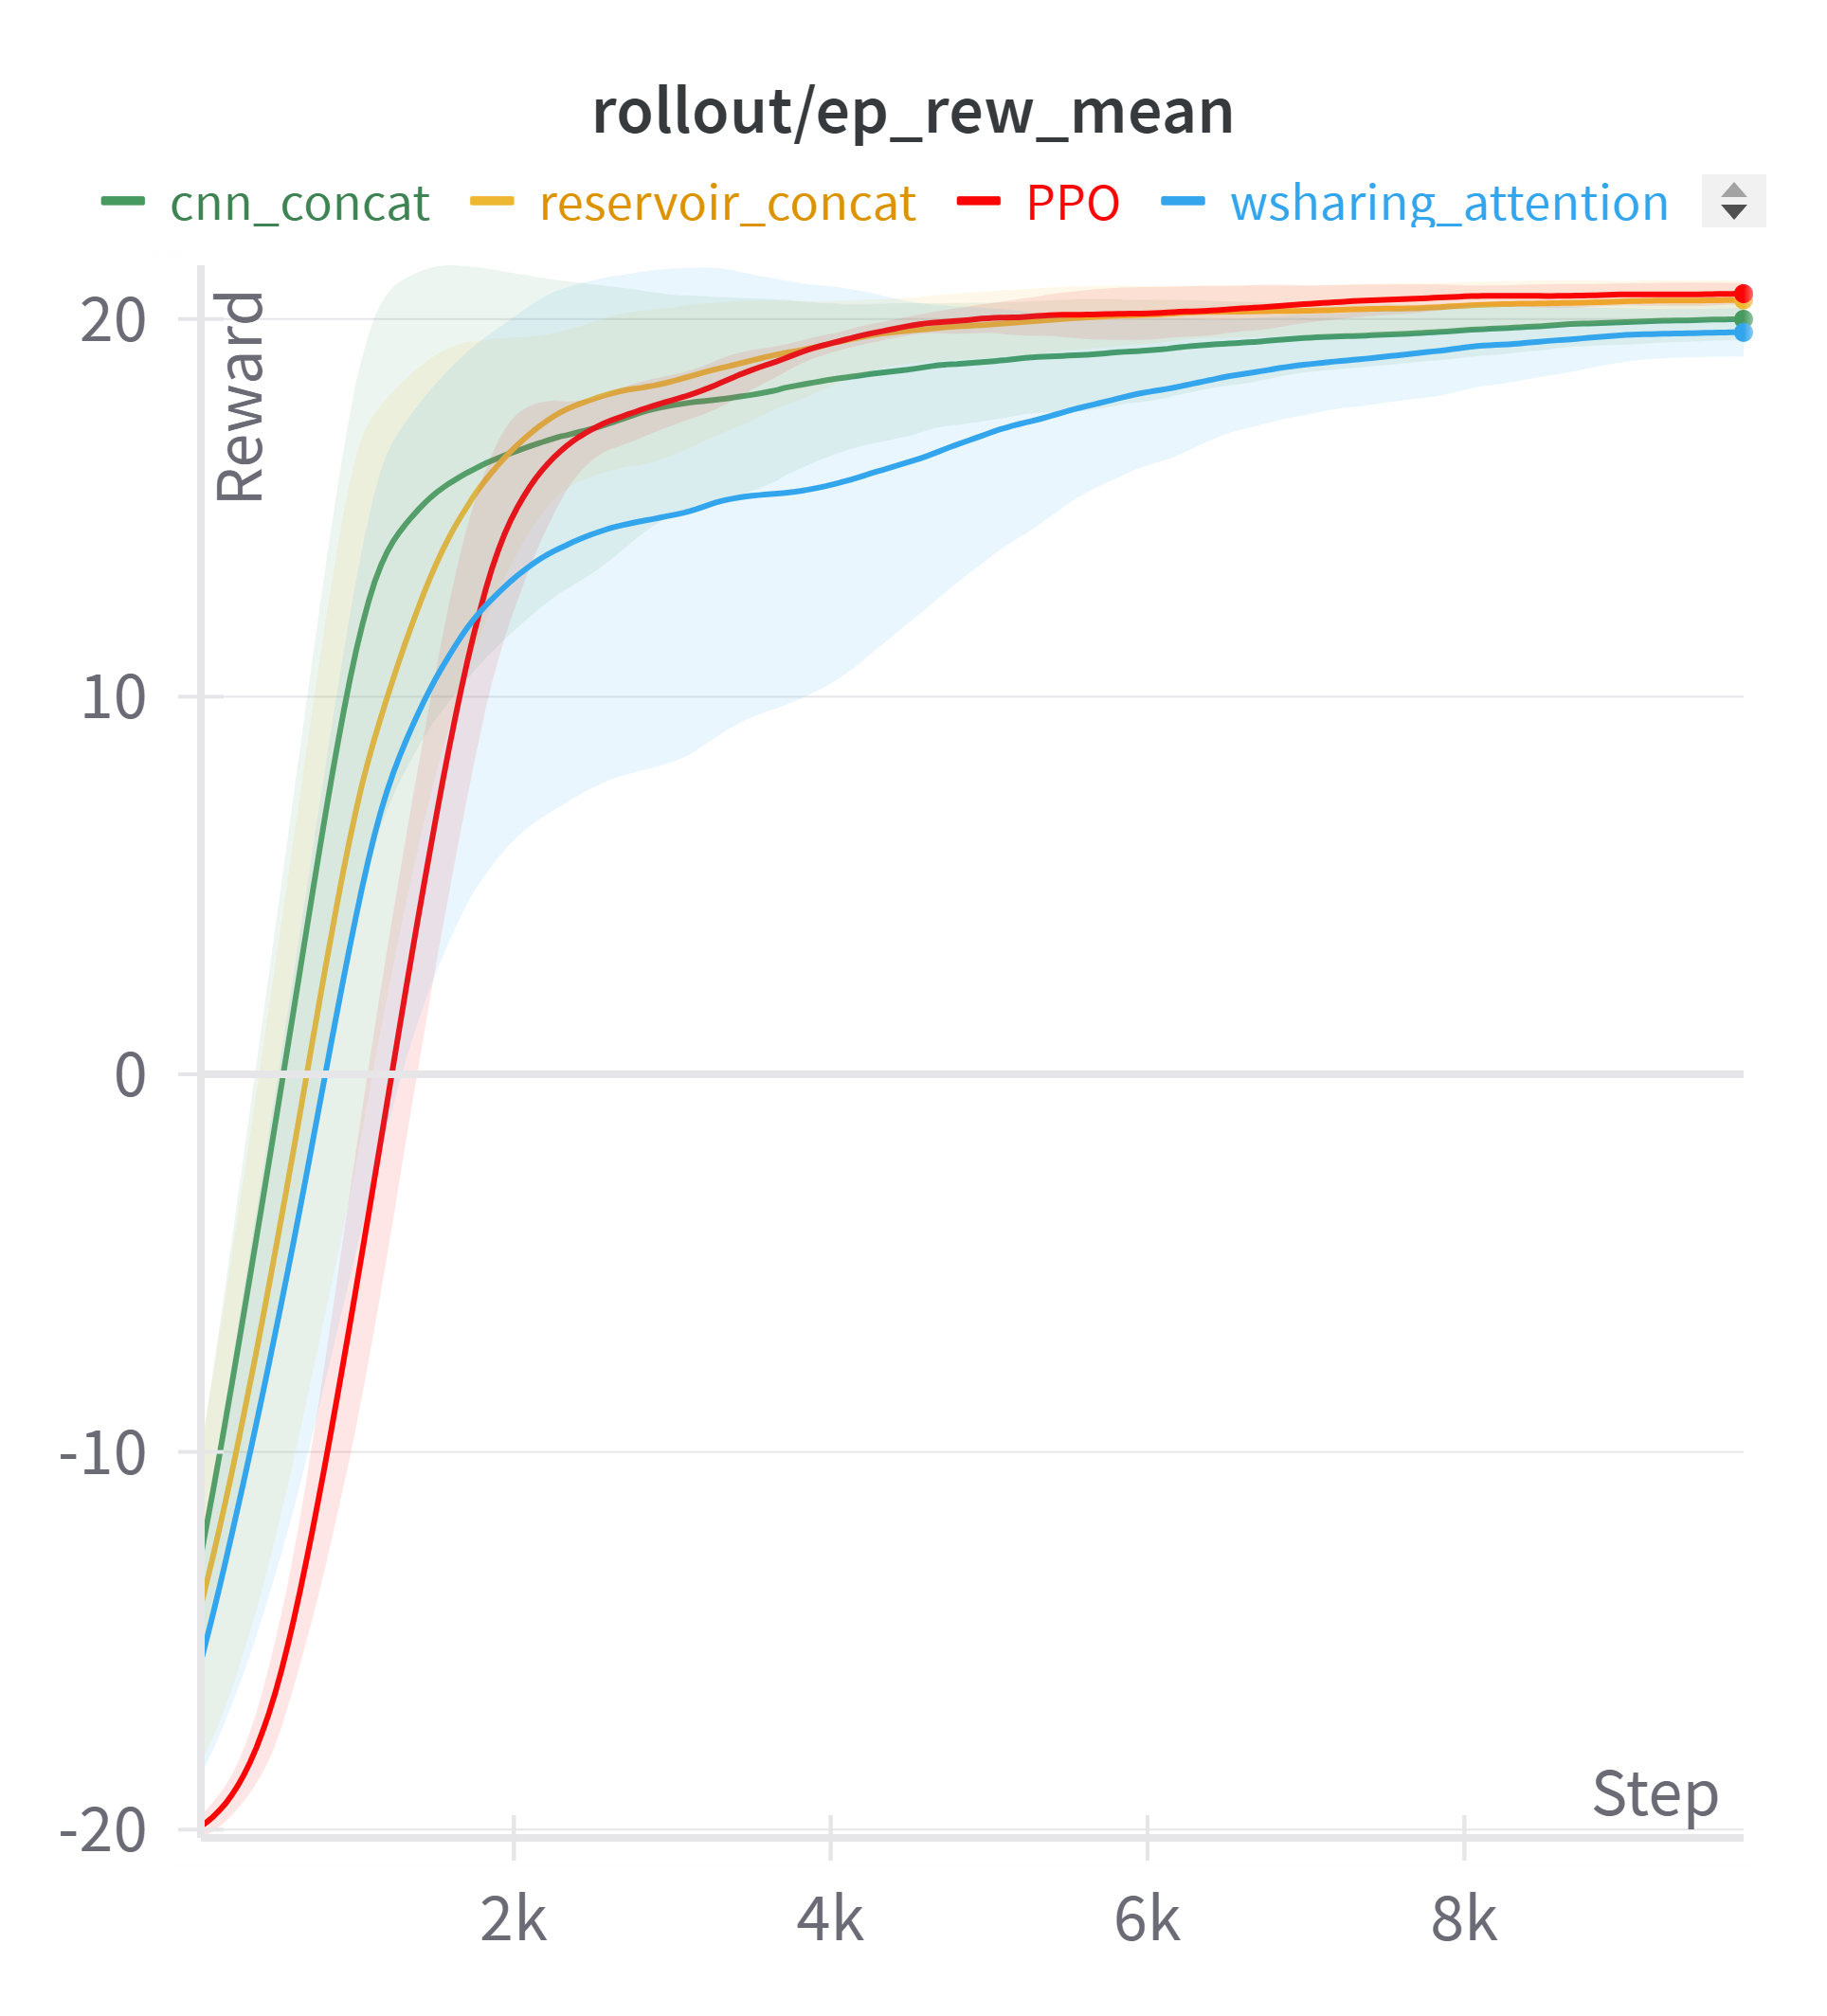
\includegraphics[width=\textwidth]{images/pong_train.png}
        \caption{Pong}
        \label{fig:pongtraining}
    \end{subfigure}
    \hfill
    \begin{subfigure}[b]{0.32\textwidth}
        \centering
        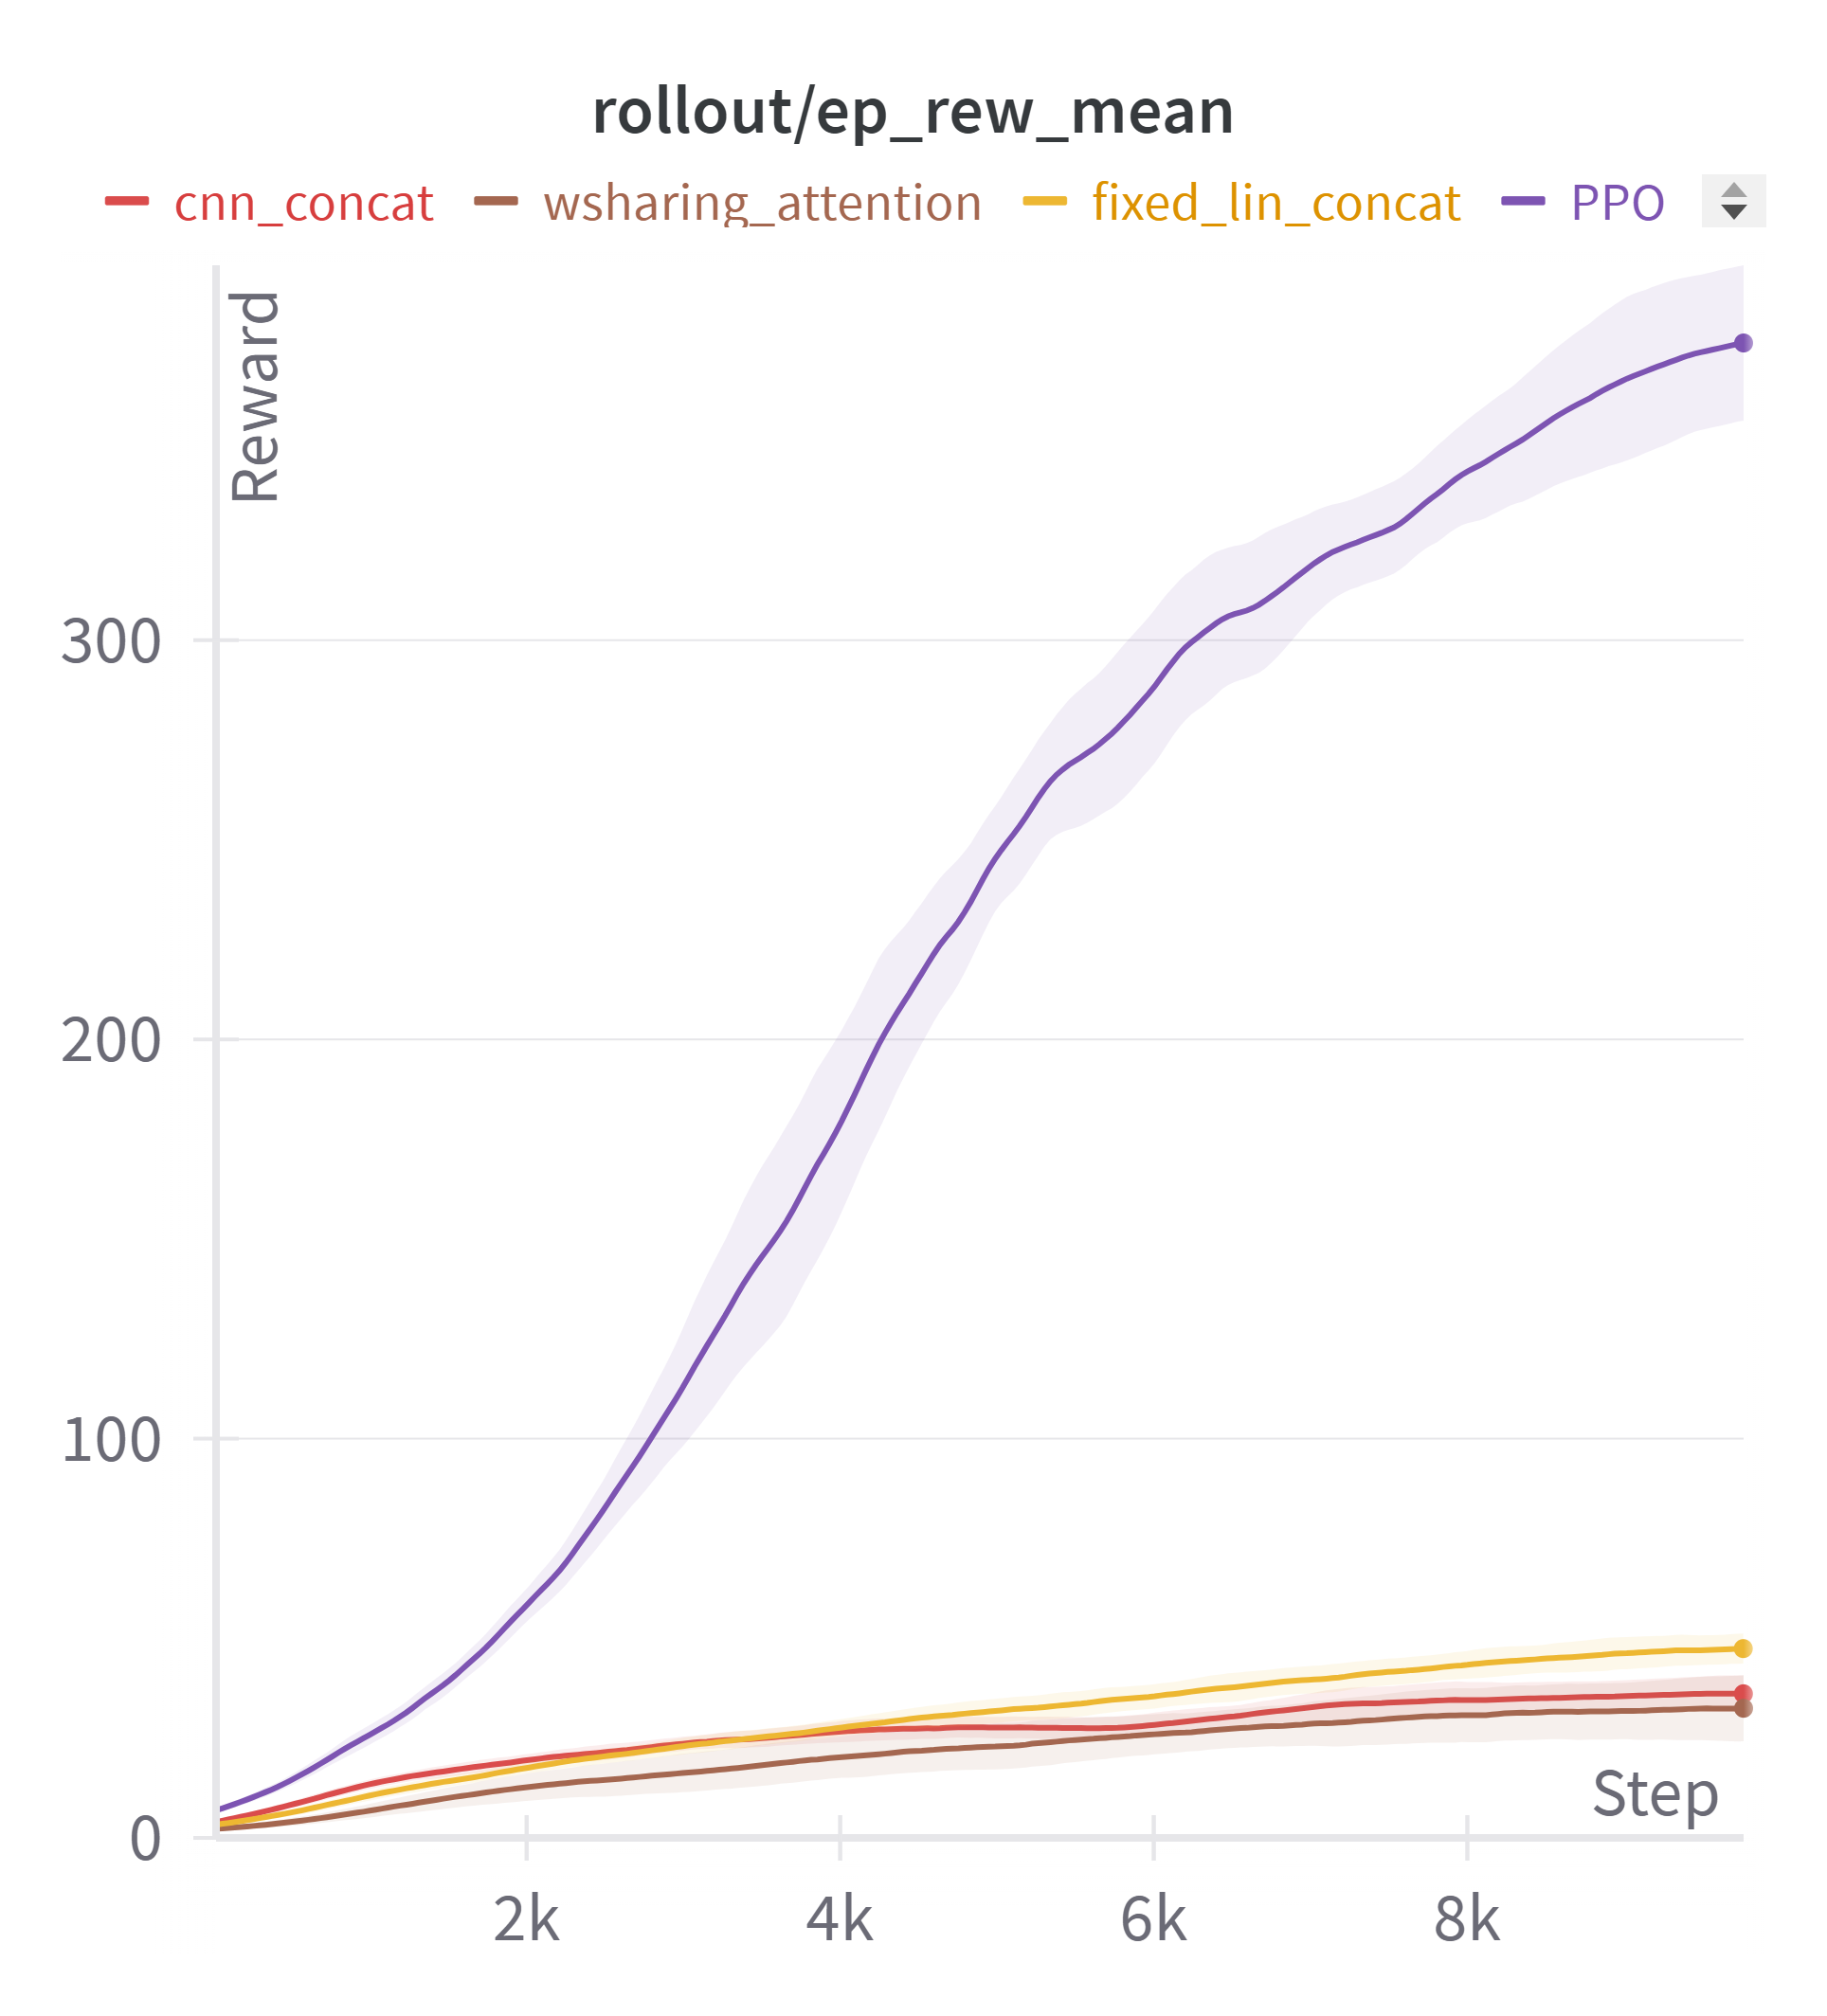
\includegraphics[width=\textwidth]{images/breakout_train.png}
        \caption{Breakout}
        \label{fig:asteroidstrain}
    \end{subfigure}
    \hfill
    \begin{subfigure}[b]{0.32\textwidth}
        \centering
        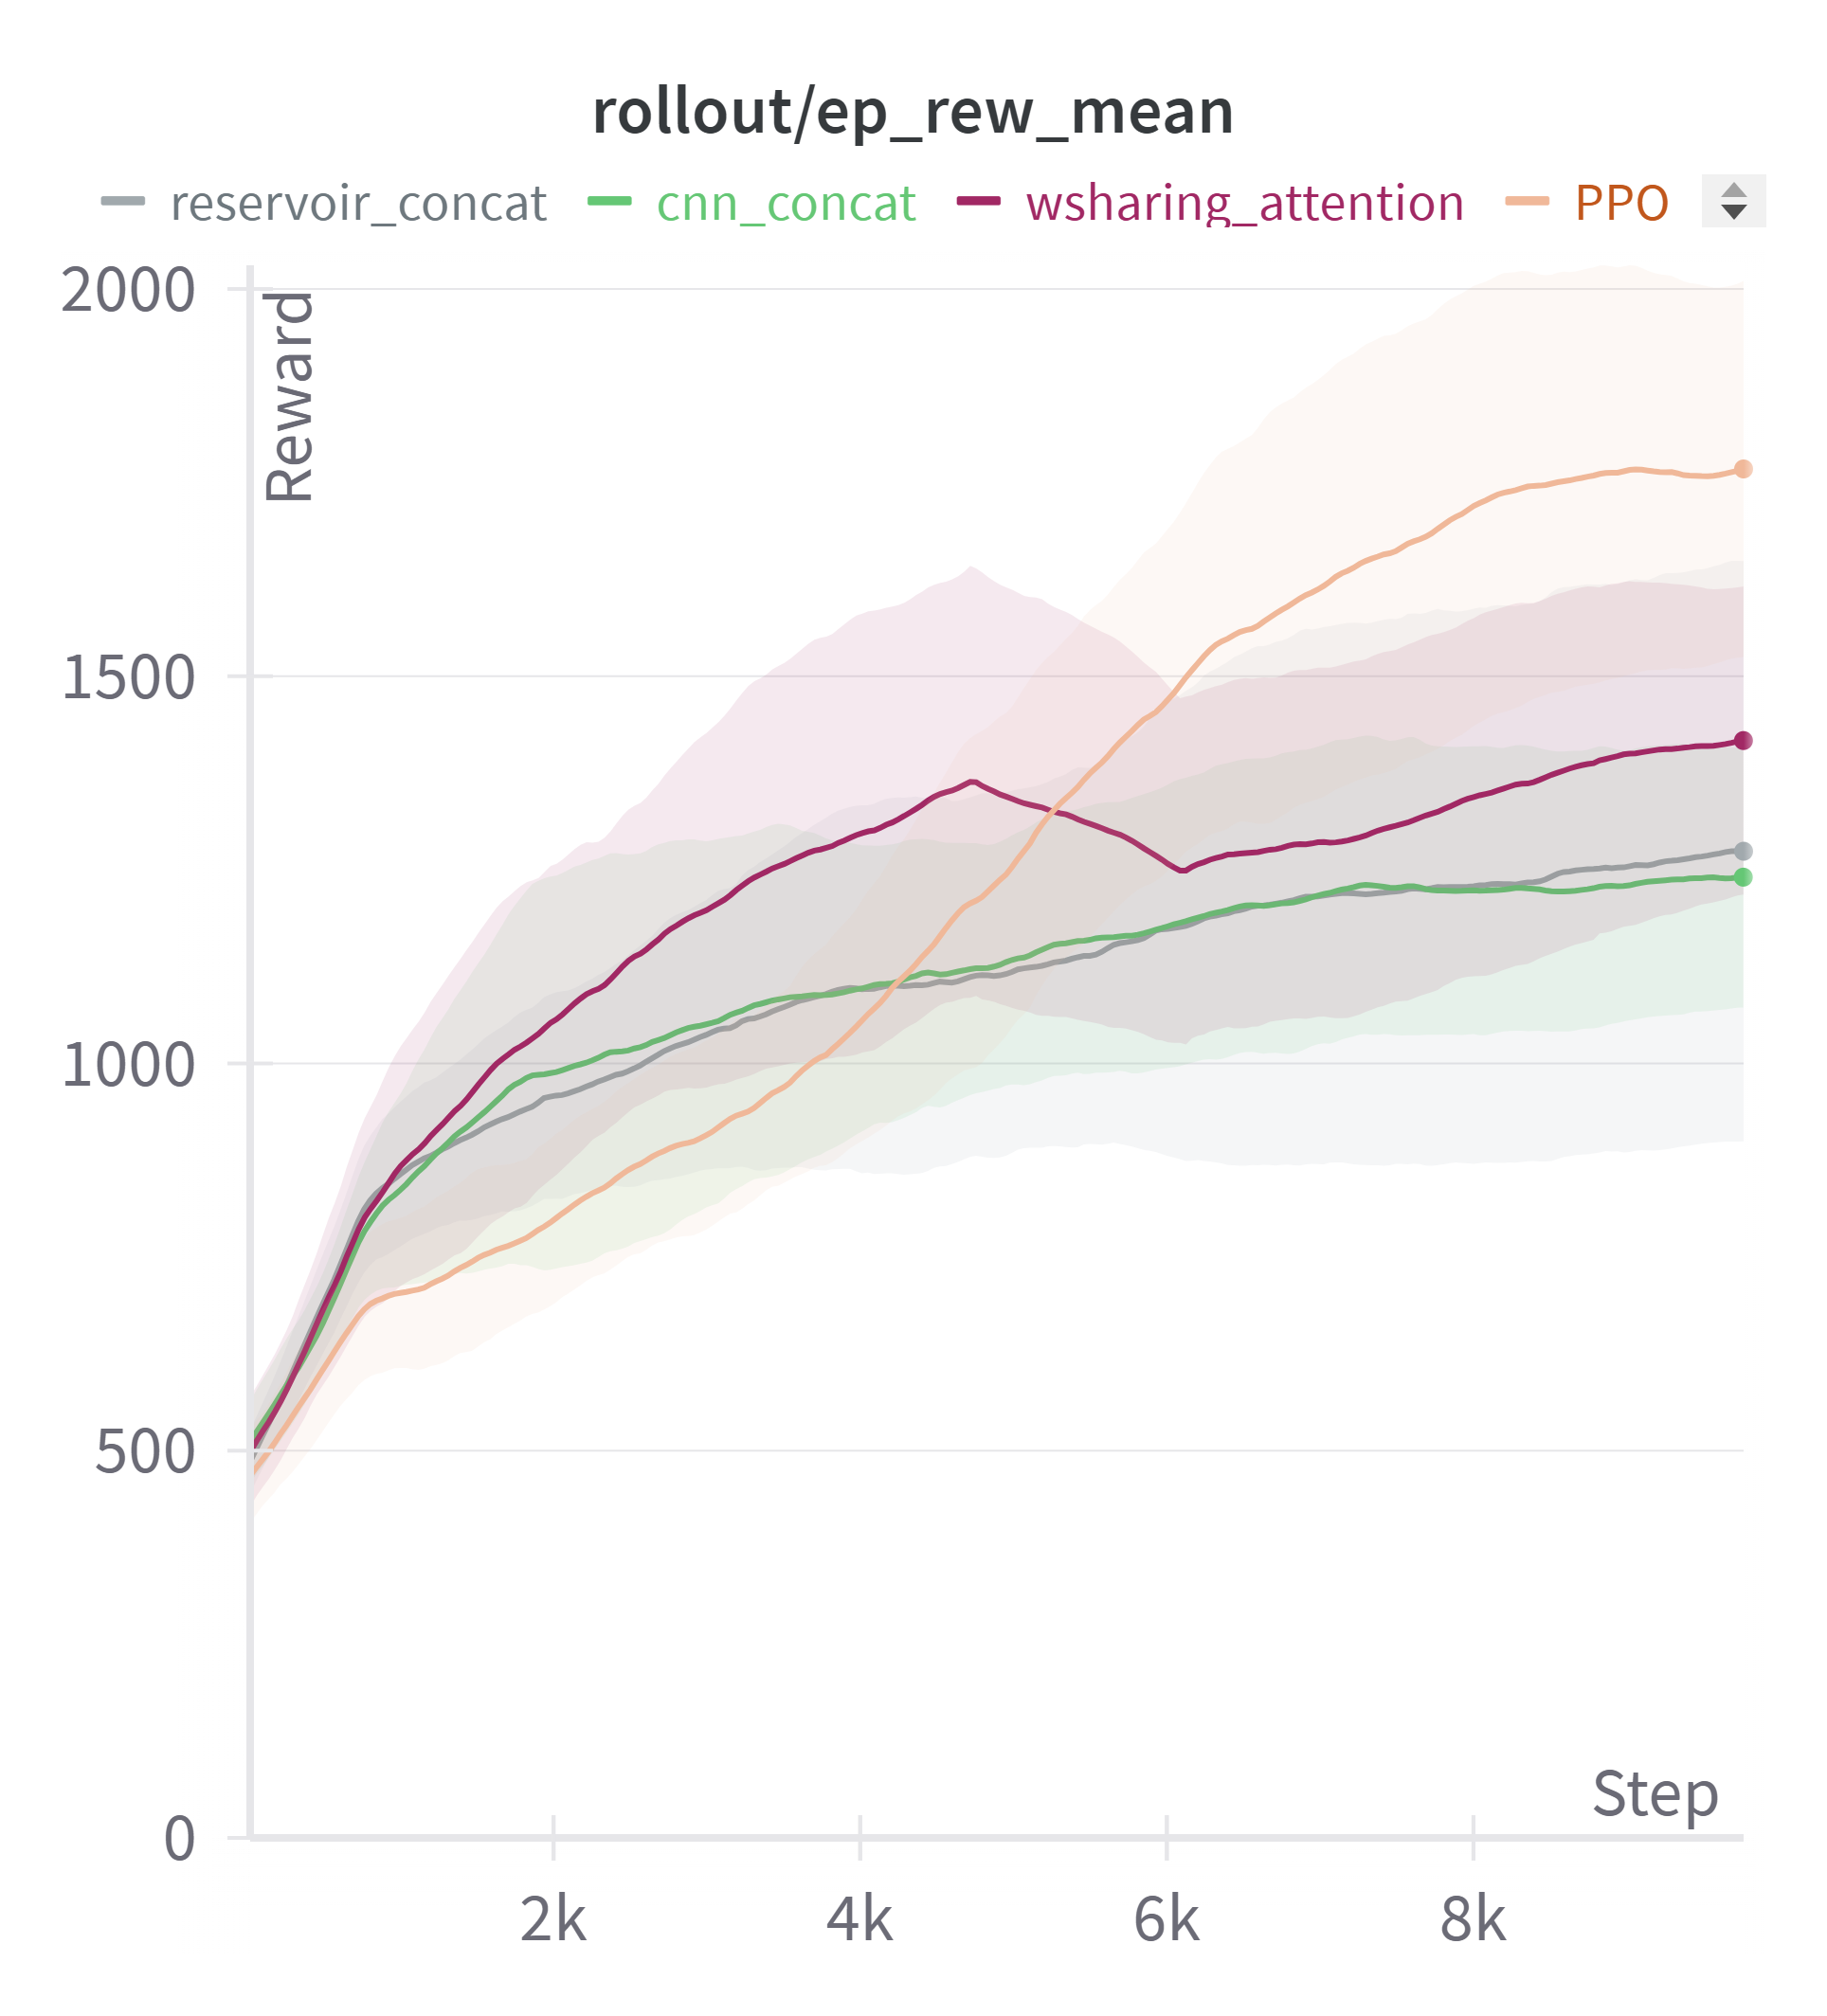
\includegraphics[width=\textwidth]{images/mspacman_train.png}
        \caption{Ms. Pacman}
        \label{fig:mspacmantrain}
    \end{subfigure}

    \caption{write caption}
    \label{fig:trainresults}
\end{figure}


As can be seen from the graphs of the learning curves, in some cases such as Pong and Ms. Pacman, the various skilled agents manage to learn faster than standard PPO. Meanwhile, in Asteroids, the learning speed is comparable with PPO.
The chosen skills track moving objects and are very useful in games such as Pong whose underlying environment does not change as the game progresses, this allows the agent to learn faster by concentrating only on the moving ball and moving bars instead of the whole game frame.

%analisi su breakout
Regarding Breakout, an initial analysis of the experiments performed shows that skill-equipped agents are not competitive with a PPO agent. This could be for various reasons, such as the fact that the skills are only trained on frames where the agent plays randomly, and as Breakout is a game where the structure changes as it progresses when the bricks are destroyed, the skills may no longer be informative in the middle or final stages of the game and even confuse the agent.
Another reason could be the fact that the skills used so far mostly track moving objects, which in Breakout are the ball and the bar. The agent may therefore have little or no information about the bricks, which are a static part of the frame.
One more reason could be that the policy learning part of the algorithm was untouched and bigger networks may extract more information from the skills.

To this end, we have made other experiments by first collecting a dataset of 1000 episodes, 500 of which are frames of an agent that plays random while the other 500 are collected using a trained PPO agent. In this way, we added variety to the dataset and we trained again the skills using this new data. We refer to these skills as \textbf{expert skills}.
As extractors, we restricted the tests only to the use of Weights Sharing with sizes 1024 and 256, as these are the ones that performed best in the other experiments, we then chose for comparison Reservoir extractor with size 1024 and Combine. We also decided to focus only on a subset of extractors to decrease the testing time.
The results of this experiment can be seen in Fig. \ref{fig:breakout_expert}

Next, we ran another experiment using expert skills and also increasing the policy network dimension of the algorithm. Standard PPO uses a linear layer of size 256 both for the policy network and value function network, we instead increased this network using three linear layers of size 1024, 512, and 256 respectively for the first, second, and third one. We use ReLU as activation function after each linear layer to add non-linearity.
The results are shown in Fig \ref{fig:breakout_expert_and_policy}.

Finally, the last round of experiments was conducted by including the skills of Image Completion and Frame Prediction in addition to the three previously used. The skills are all used in expert mode and we also increased the policy learning network as before.
For this last experiment, we used only the agent that performed best in the other experiments, namely Weights sharing with embedding dimensions 256 and 1024.
Fig. \ref{fig:breakout_expert_policy_skills} shows the results.

\begin{figure}[htbp]
    \centering
    \begin{subfigure}[b]{0.32\textwidth}
        \centering
        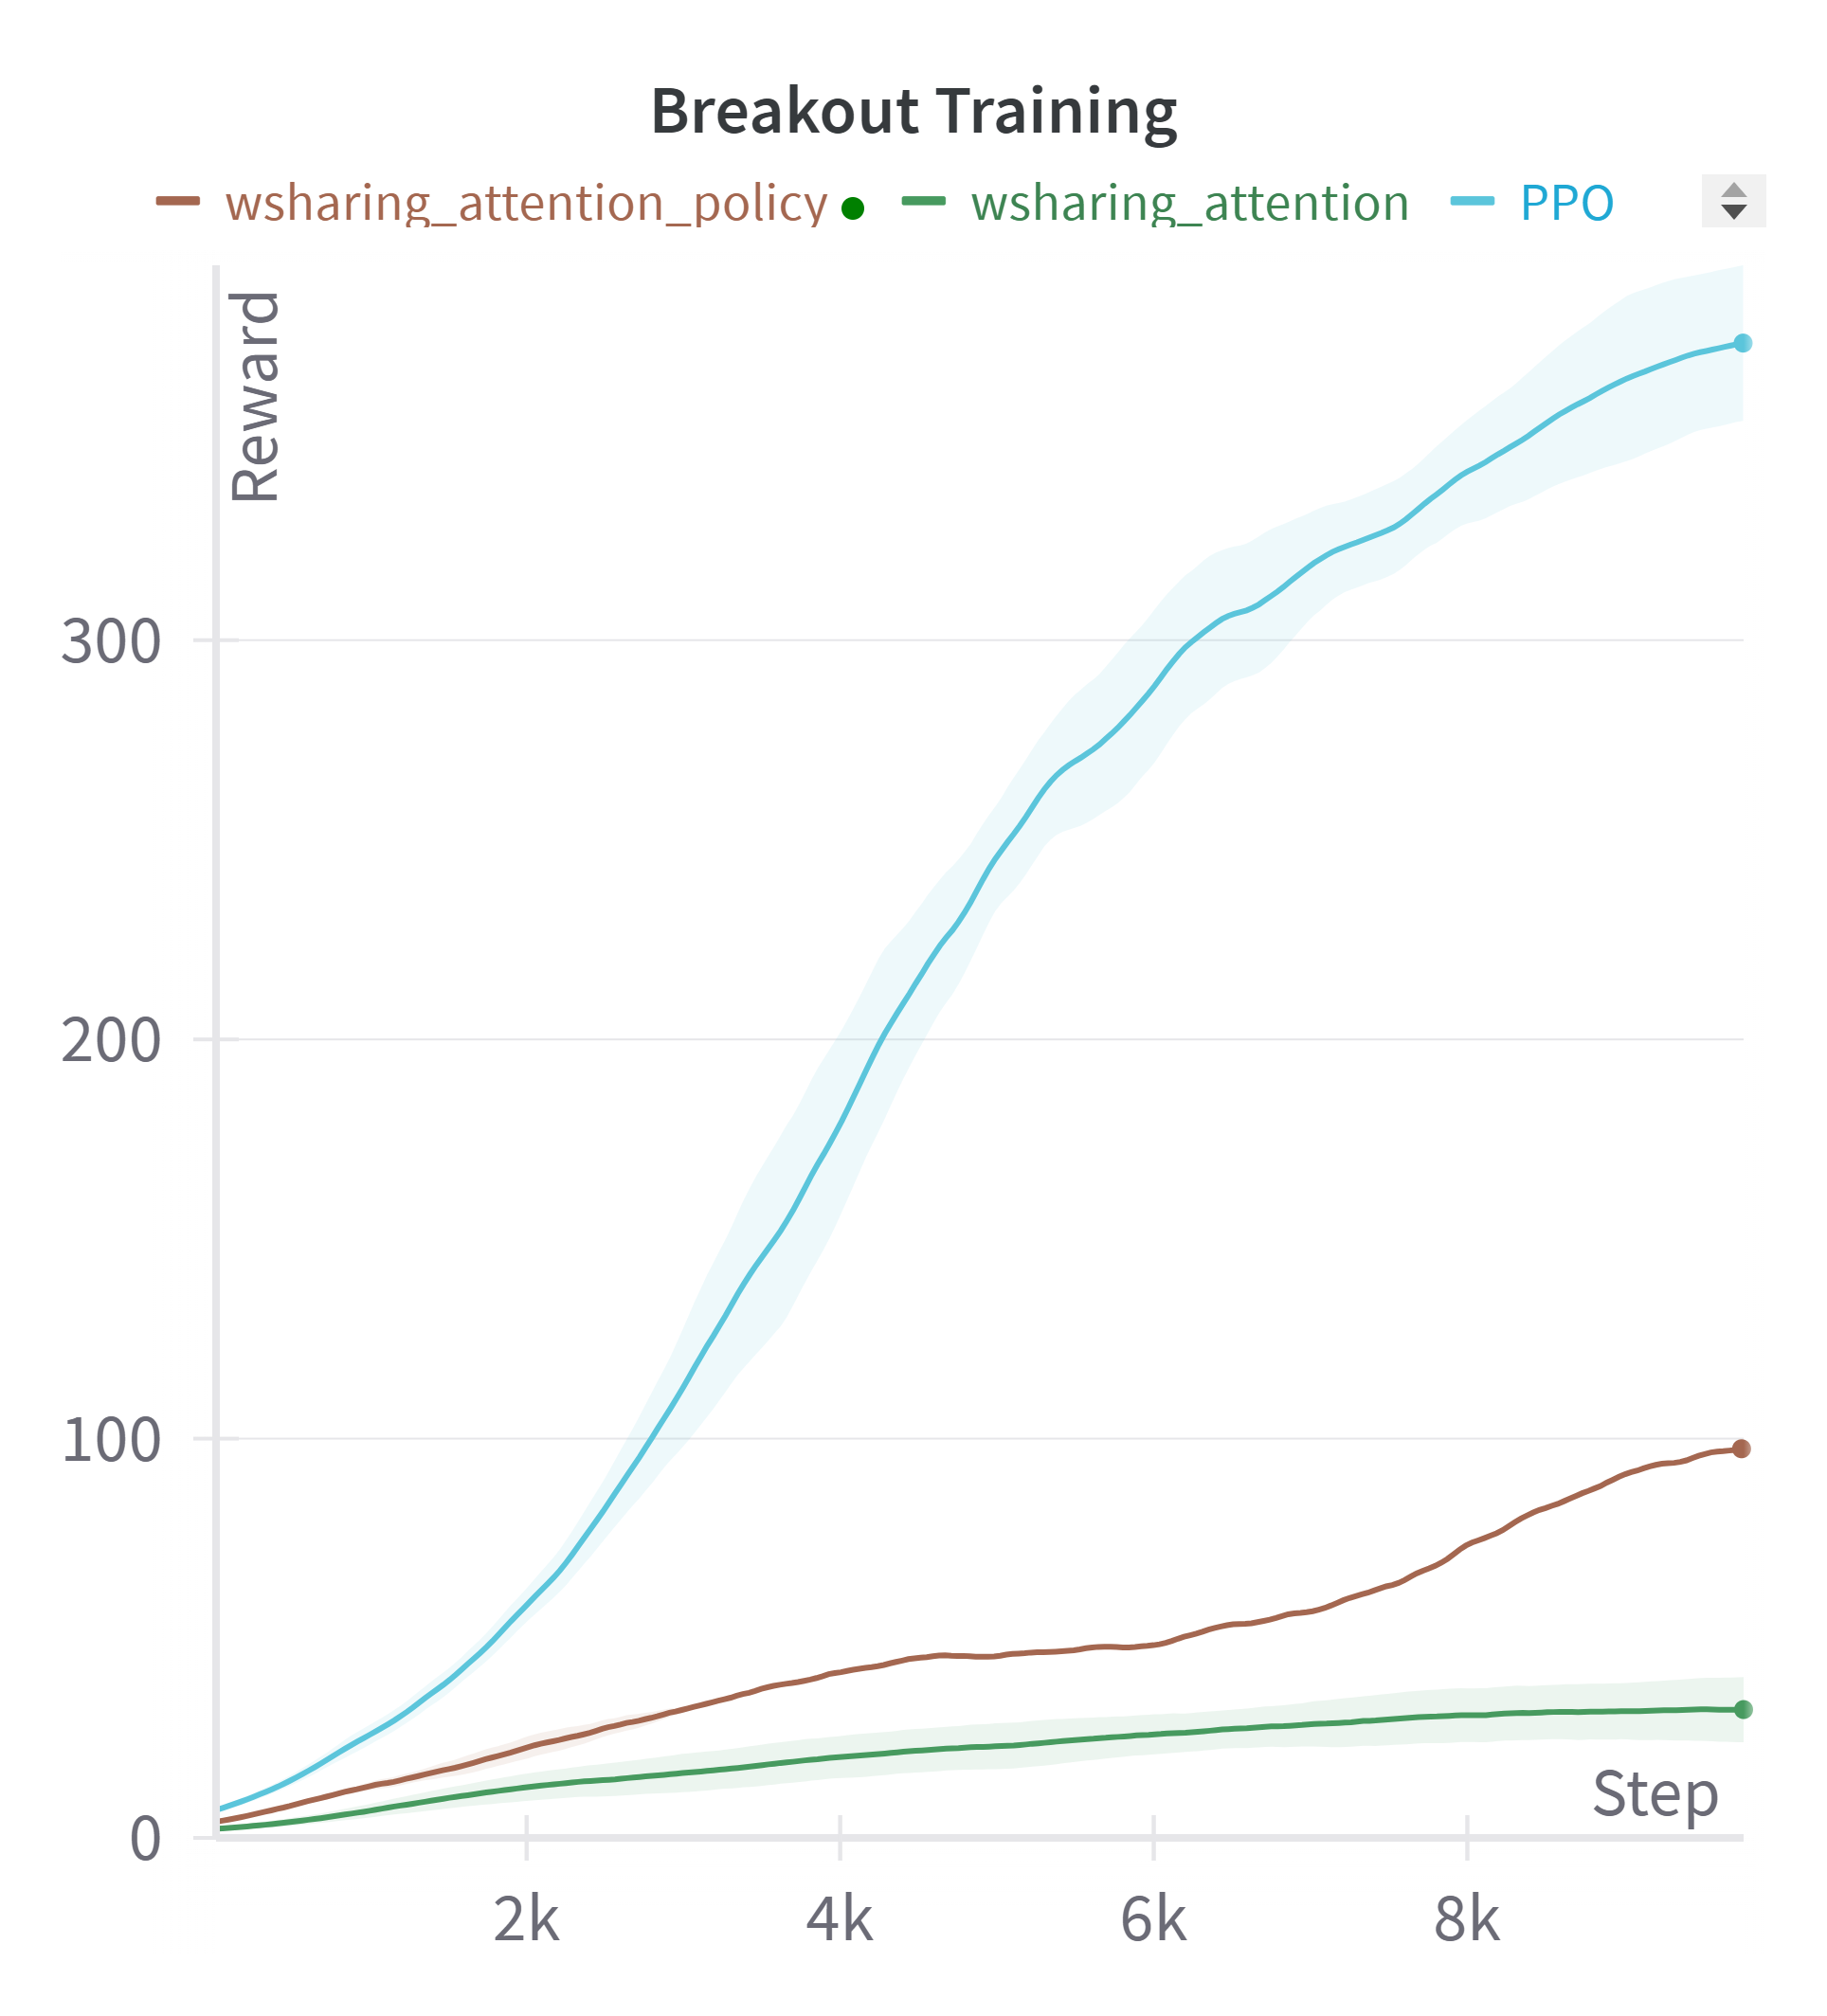
\includegraphics[width=\textwidth]{images/breakout_policy.png}
        \caption{Breakout con MLP + quello che faceva schifo}
        \label{fig:breakout_expert}
    \end{subfigure}
    \hfill
    \begin{subfigure}[b]{0.32\textwidth}
        \centering
        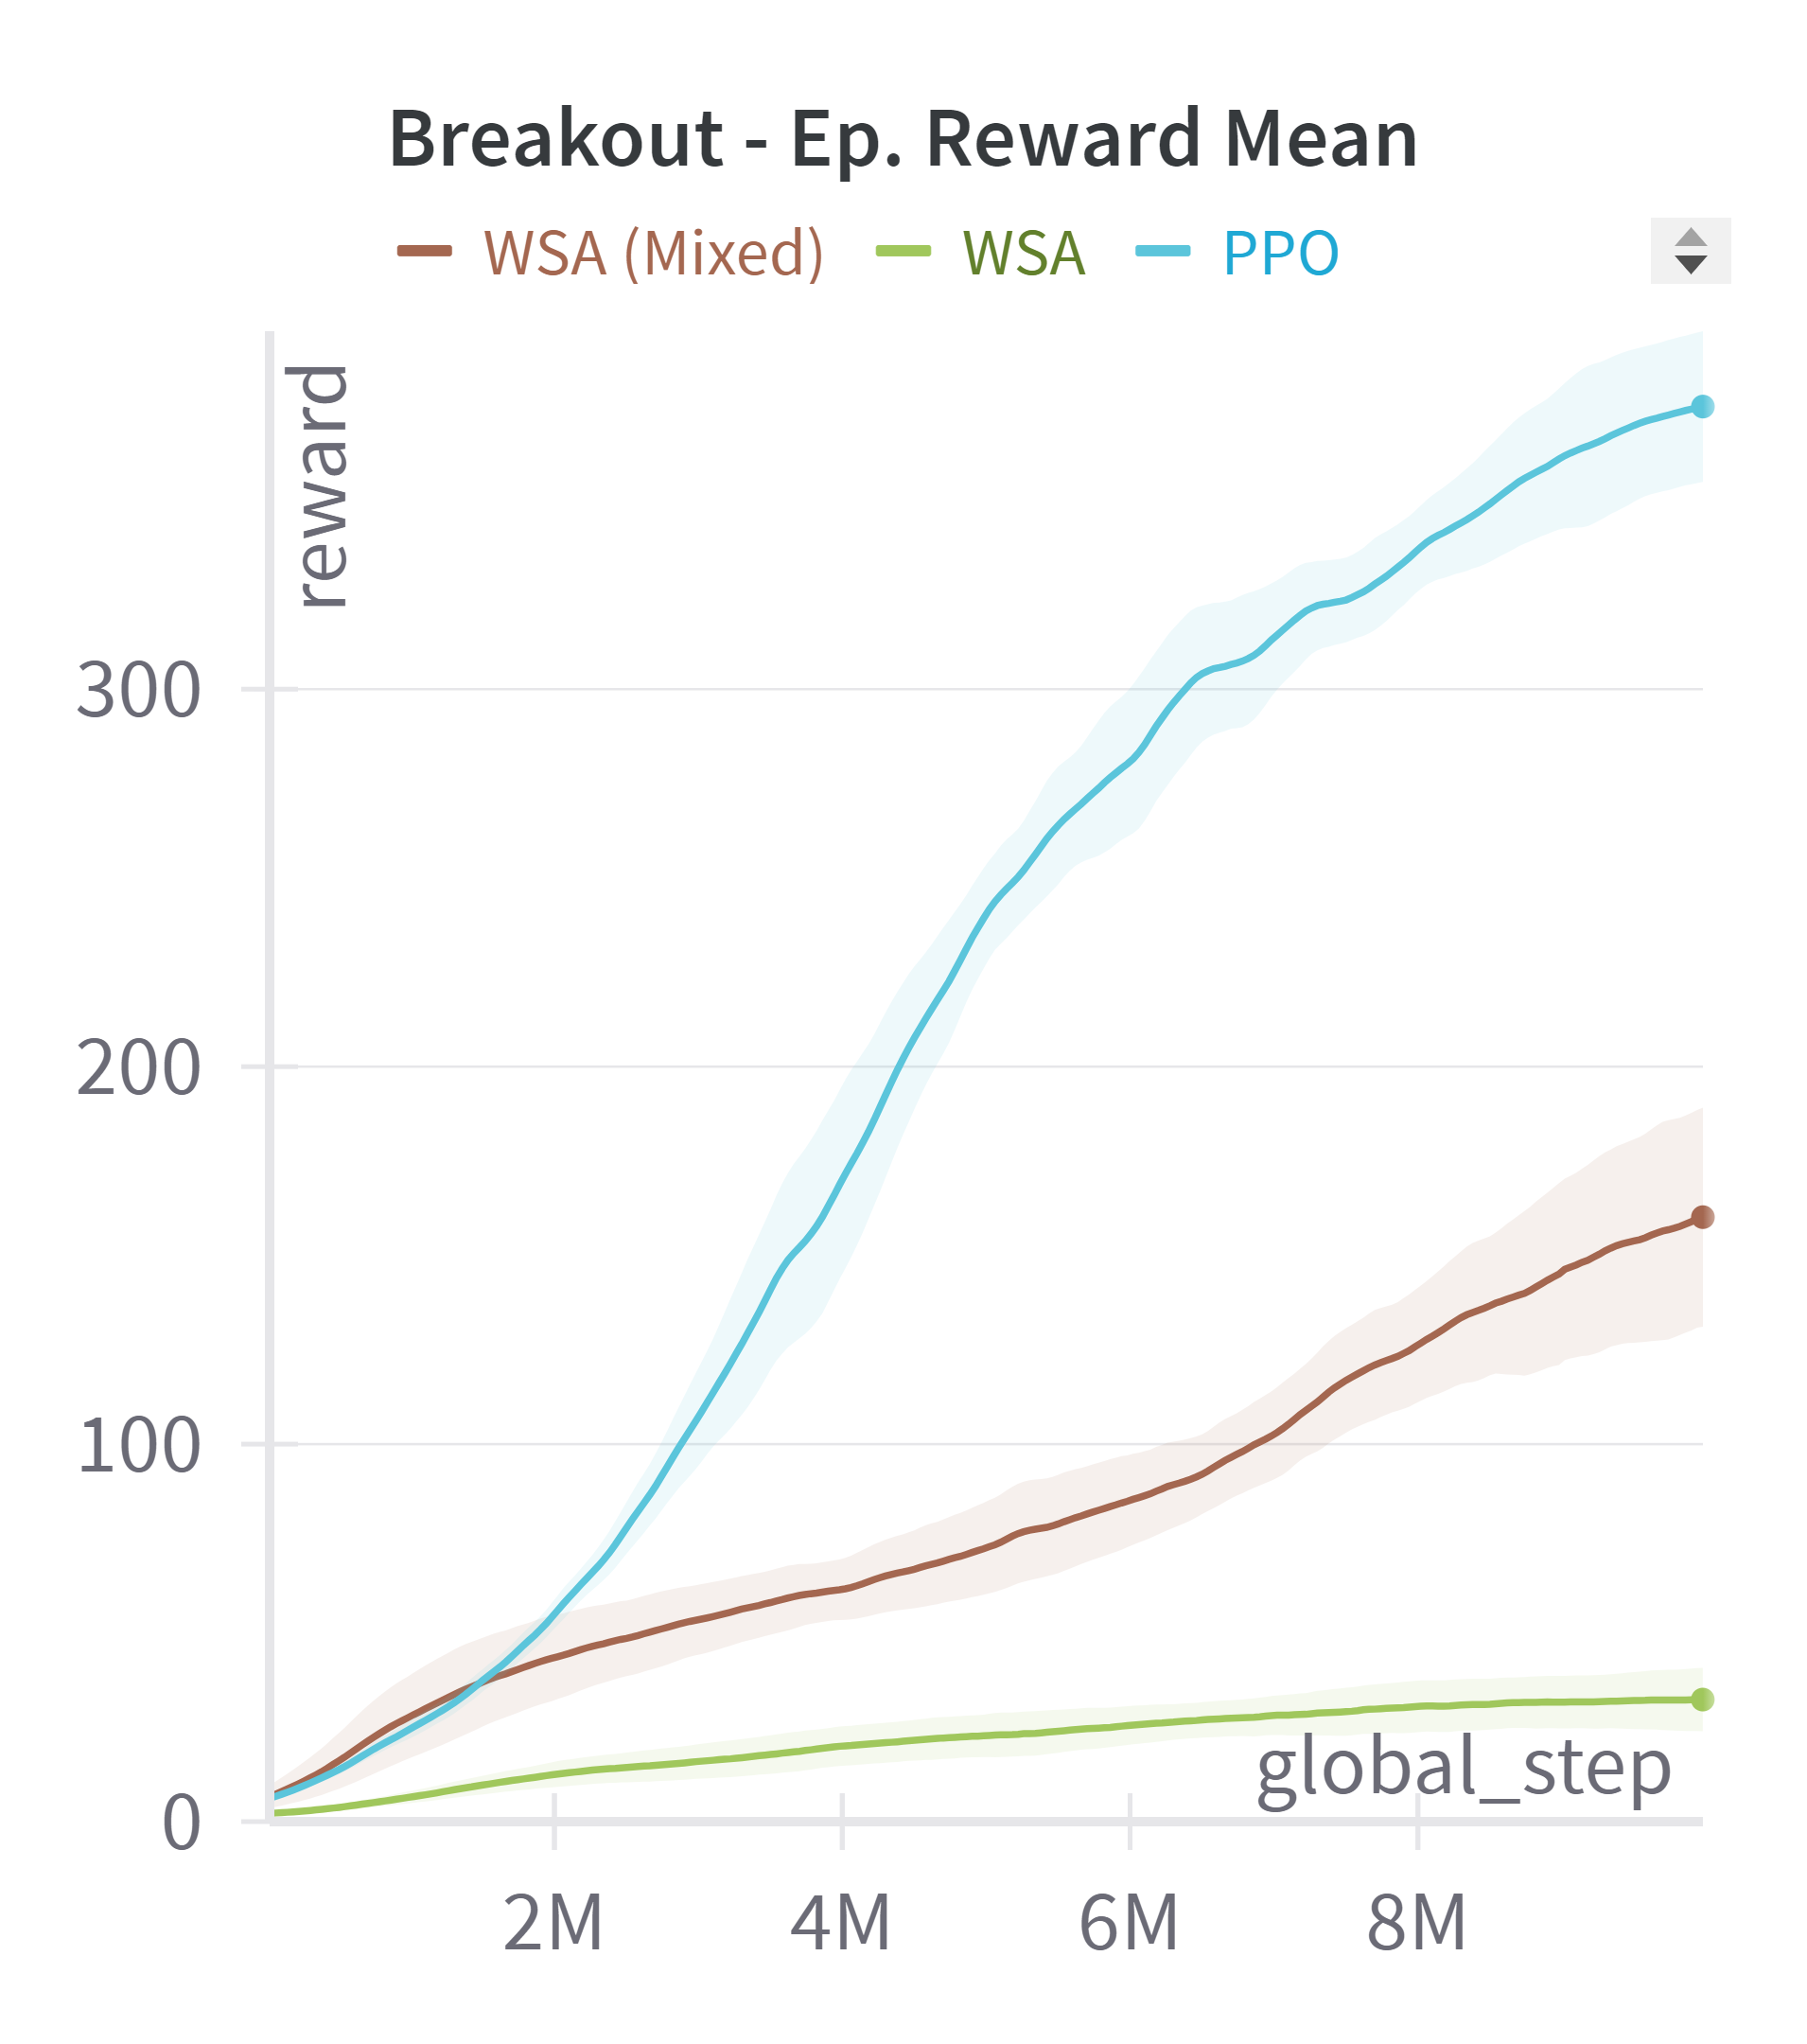
\includegraphics[width=\textwidth]{images/breakout_expert.png}
        \caption{Breakout stesso di prima ma con dati expert}
        \label{fig:breakout_expert_and_policy}
    \end{subfigure}
    \hfill
    \begin{subfigure}[b]{0.32\textwidth}
        \centering
        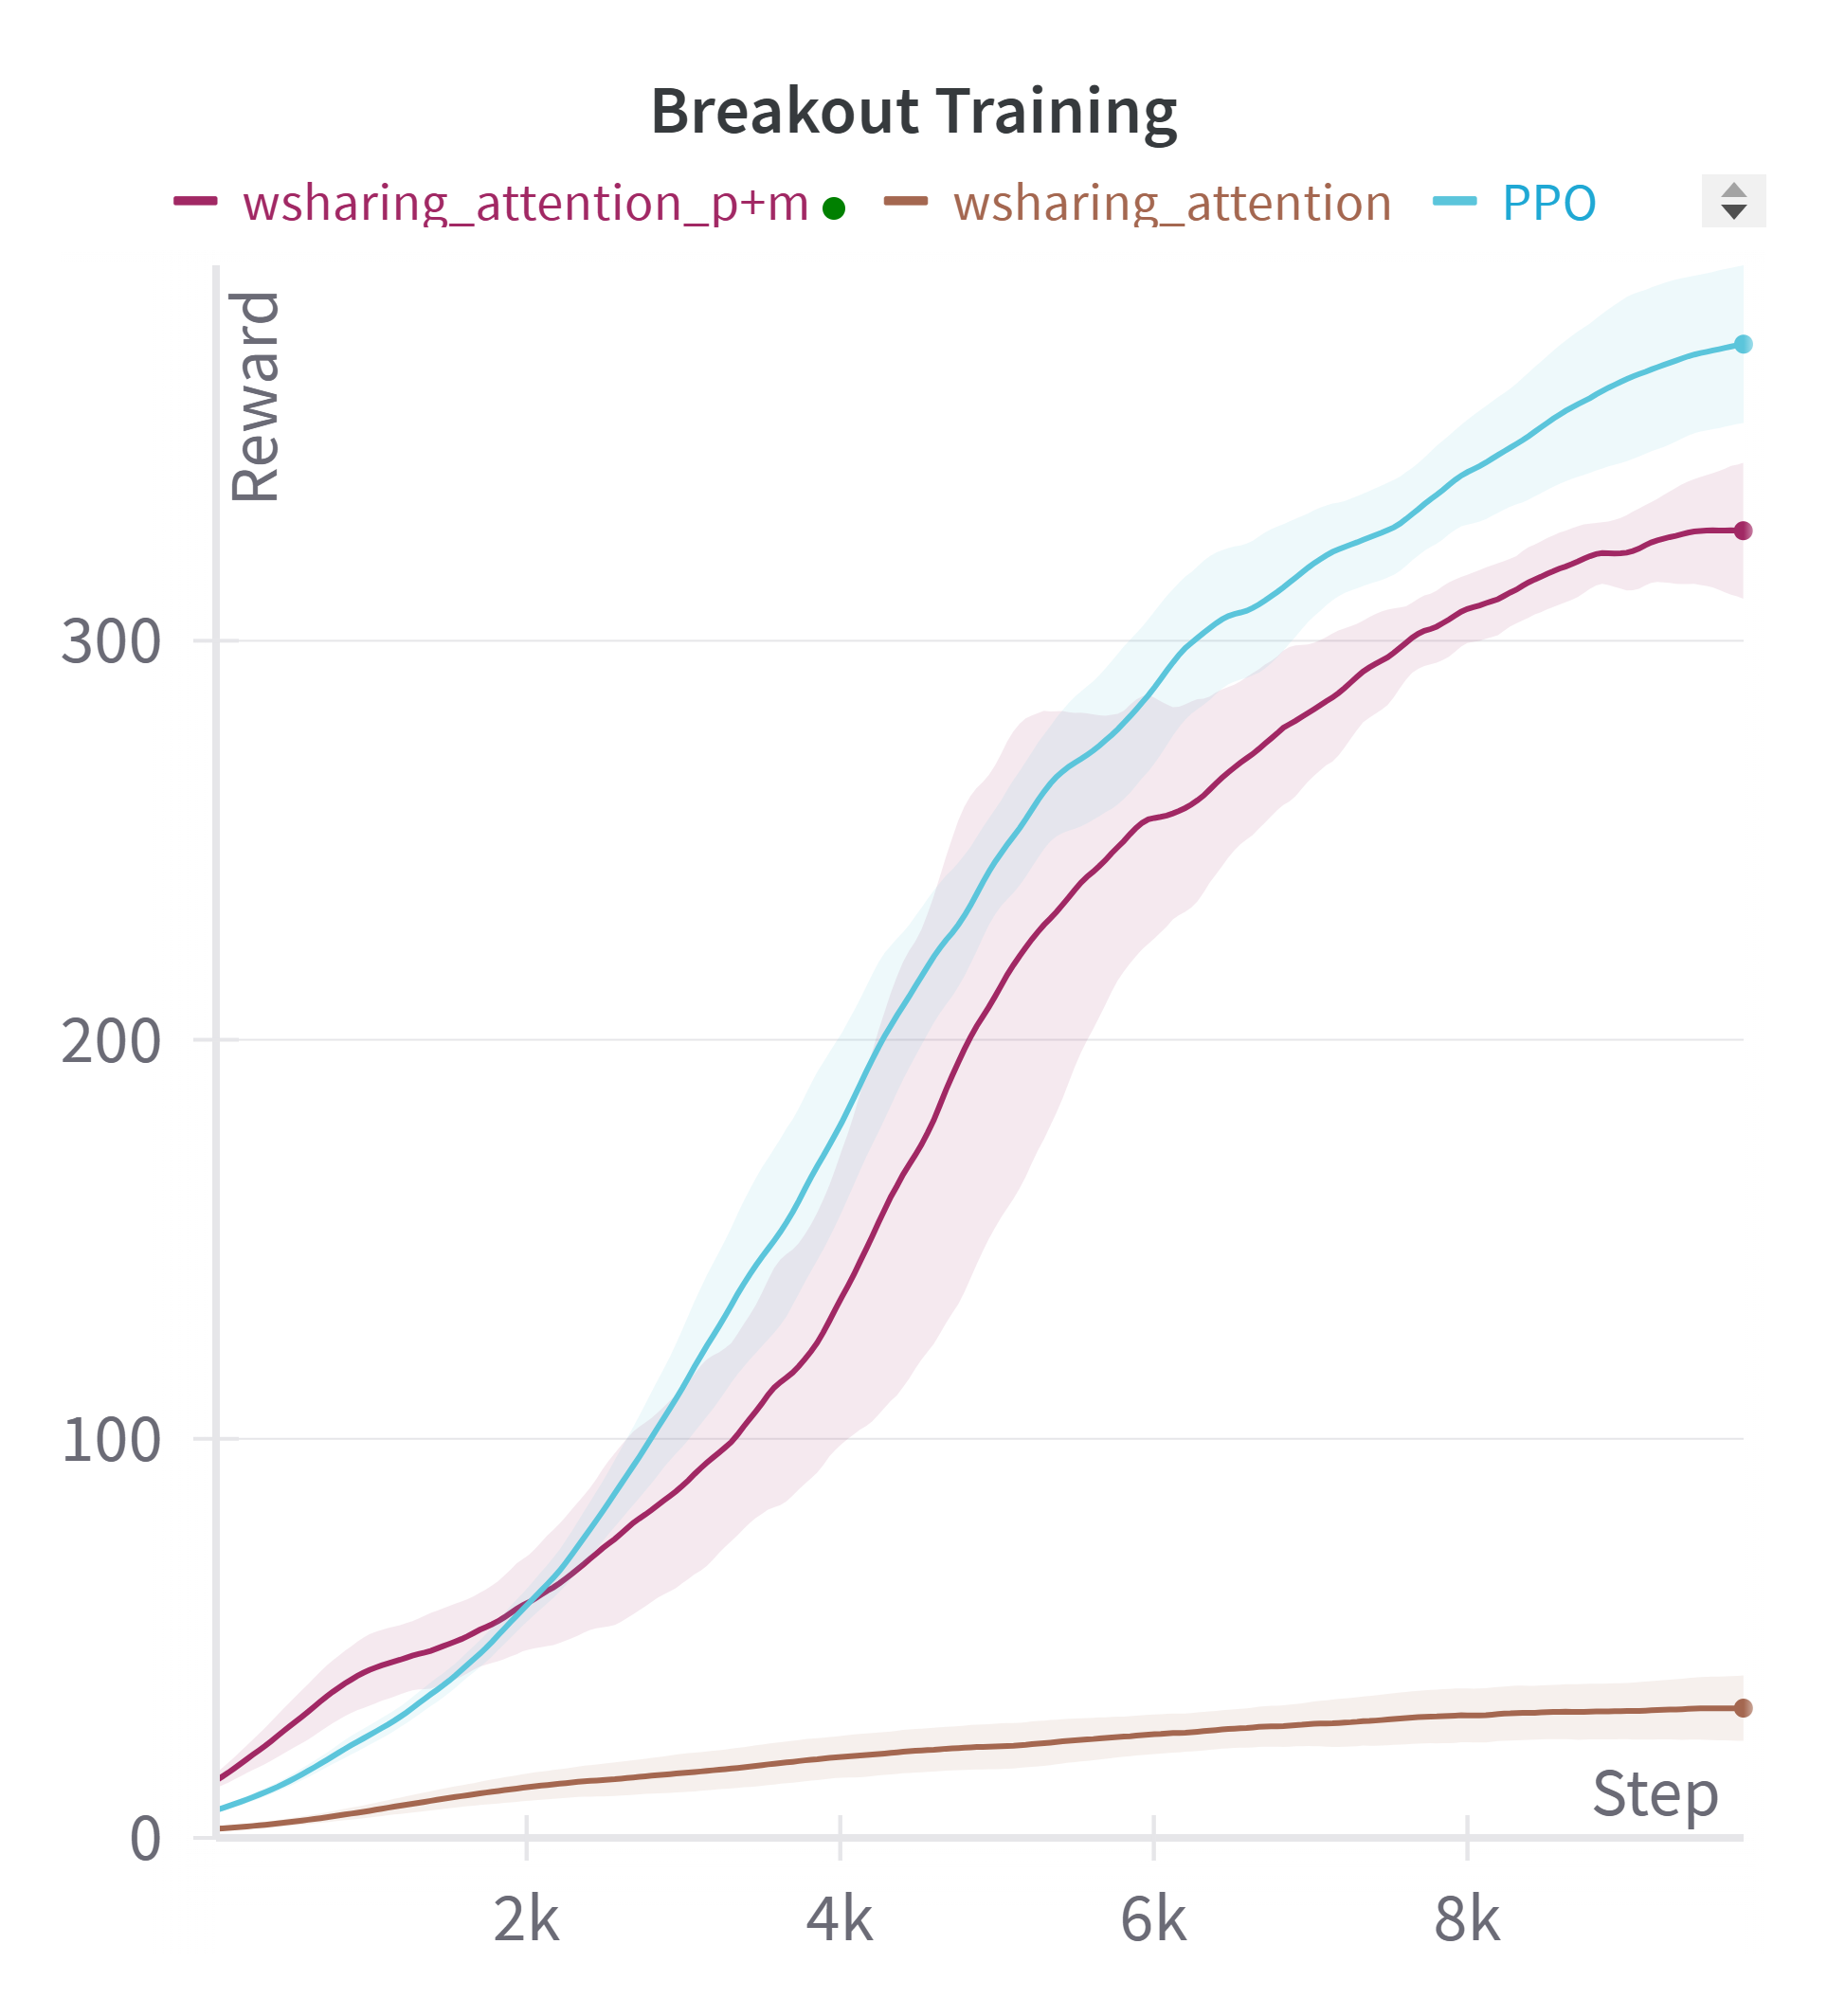
\includegraphics[width=\textwidth]{images/breakout_p+m.png}
        \caption{Breakout expert  + policy}
        \label{fig:breakout_expert_policy_skills}
    \end{subfigure}
    \hfill

    \caption{PPO
 rimane uguale in tutti e 3}
    \label{fig:trainresults}
\end{figure}



Tab. \ref{tab:results} shows the highest reward obtained for each game by the top three agents of each game considering the evaluation. This table also presents the agent called PPO which represents our training run of a standard PPO agent without skills, and the agent REFERENCE which is the result reported on the Hugging Face page of Stable-Baselines.

\begin{table}[htbp]
    \begin{center}
        \begin{tabular}{llll}
            \multicolumn{1}{l}{AGENT}  &\multicolumn{1}{l}{\bf PONG} &\multicolumn{1}{l}{\bf BREAKOUT} &\multicolumn{1}{l}{\bf MS. PACMAN}
            \\ \hline \\
            Weights Sharing (1024) &  20 $\pm$ 00 &  - &  -  \\
            Weights Sharing (256)  &  - &  356 $\pm$ 00 &  2487 $\pm$ 00  \\
            Reservoir (1024)       &  20 $\pm$ 00 &  - &  2111 $\pm$ 00 \\
            CNN (2)                &  20 $\pm$ 00 &  - &  1812 $\pm$ 00 \\
            CNN (3)                &  - &  50 $\pm$ 00 &  - \\
            Fixed Lin. (512)                &  - &  50 $\pm$ 00 &  - \\
            PPO                    &  20 $\pm$ 00 &  387 $\pm$ 00 &  2230 $\pm$ 00 \\
            REFERENCE              &  21 $\pm$ 0 &  398 $\pm$ 16.30 &  1659 $\pm$ 144.81 \\
        \end{tabular}
    \end{center}
    \caption{Tra parentesi le dimensioni}
    \label{tab:results}
\end{table}

%As can be seen in \ref{fig:breakout_expert} we tested Breakout with expert skills only on a subset of a few extractors. We chose Weights Sharing Attention with 256 and 1024 as dimensions for skills embeddings, Combine Extractor, and Reservoir Extractor with 1024 as dimension of the reservoir. We restricted only to these extractors to increase the time for experiments too much.
%We can see that only by using expert skills the Weights Sharing agent become comparable with the PPO agent, it learns more slowly but eventually in evaluation manages to have a score very similar to PPO. Reaching xxx while PPO reaches xxx.

%Let us now analyze the use of expert skills and the increase of the network involved in policy learning.
%We can see in Fig. \ref{fig:breakout_expert_and_policy} that Weights Sharing Attention with dimension 256 for skills embeddings is the one that performs the best. It is comparable with a PPO agent since they perform basically the same.

%Finally, for what regards the use of more skills in Fig. \ref{fig:breakout_expert_policy_skills} we can see ...


%analisi weights sharing
%In most of the experiments we have performed, we have noticed that weights sharing attention as a way of concatenating different skill embeddings is the one that performs best.
%It, being more general as a method manages to better filter out noisy input, focusing only on the information that is really important for the agent to learn.
INSERIRE ANALISI WEIGHTS SHARING
Lorem Ipsum is simply dummy text of the printing and typesetting industry. Lorem Ipsum has been the industry's standard dummy text ever since the 1500s, when an unknown printer took a galley of type and scrambled it to make a type specimen book. It has survived not only five centuries, but also the leap into electronic typesetting, remaining essentially unchanged. It was popularised in the 1960s with the release of Letraset sheets containing Lorem Ipsum passages, and more recently with desktop publishing software like Aldus PageMaker including versions of Lorem Ipsum

INSERIRE ANALISI SUL NUMERO DI PARAMETRI TOTALI DI PPO E SKILLED AGENT
Lorem Ipsum is simply dummy text of the printing and typesetting industry. Lorem Ipsum has been the industry's standard dummy text ever since the 1500s, when an unknown printer took a galley of type and scrambled it to make a type specimen book. It has survived not only five centuries, but also the leap into electronic typesetting, remaining essentially unchanged. It was popularised in the 1960s with the release of Letraset sheets containing Lorem Ipsum passages, and more recently with desktop publishing software like Aldus PageMaker including versions of Lorem Ipsum

INSERIRE ANALISI SUGLI FPS TRA PPO E SKILLED AGENT
Lorem Ipsum is simply dummy text of the printing and typesetting industry. Lorem Ipsum has been the industry's standard dummy text ever since the 1500s, when an unknown printer took a galley of type and scrambled it to make a type specimen book. It has survived not only five centuries, but also the leap into electronic typesetting, remaining essentially unchanged. It was popularised in the 1960s with the release of Letraset sheets containing Lorem Ipsum passages, and more recently with desktop publishing software like Aldus PageMaker including versions of Lorem Ipsum

